%%%%%%%%%%%%%%%%%%%%%%% file template.tex %%%%%%%%%%%%%%%%%%%%%%%%%
%
% This is a general template file for the LaTeX package SVJour3
% for Springer journals.          Springer Heidelberg 2010/09/16
%
% Copy it to a new file with a new name and use it as the basis
% for your article. Delete % signs as needed.
%
% This template includes a few options for different layouts and
% content for various journals. Please consult a previous issue of
% your journal as needed.
%
%%%%%%%%%%%%%%%%%%%%%%%%%%%%%%%%%%%%%%%%%%%%%%%%%%%%%%%%%%%%%%%%%%%
%
% First comes an example EPS file -- just ignore it and
% proceed on the \documentclass line
% your LaTeX will extract the file if required
\begin{filecontents*}{example.eps}
\usepackage[numbers, square, sectionbib]{natbib}

%!PS-Adobe-3.0 EPSF-3.0
%%BoundingBox: 19 19 221 221
%%CreationDate: Mon Sep 29 1997
%%Creator: programmed by hand (JK)
%%EndComments
gsave
newpath
  20 20 moveto
  20 220 lineto
  220 220 lineto
  220 20 lineto
closepath
2 setlinewidth
gsave
  .4 setgray fill
grestore
stroke
grestore
\end{filecontents*}
%
\RequirePackage{fix-cm}
%
%\documentclass{svjour3}                     % onecolumn (standard format)
%\documentclass[smallcondensed]{svjour3}     % onecolumn (ditto)
\documentclass[smallextended]{svjour3}       % onecolumn (second format)
%\documentclass[twocolumn]{svjour3}          % twocolumn
%
\smartqed  % flush right qed marks, e.g. at end of proof
%
\usepackage{graphicx}
\usepackage{apalike}
%
% \usepackage{mathptmx}      % use Times fonts if available on your TeX system
%
% insert here the call for the packages your document requires
%\usepackage{latexsym}
% etc.
%
% please place your own definitions here and don't use \def but
% \newcommand{}{}
%
% Insert the name of "your journal" with
\journalname{Journal of Visualization}
%
\begin{document}

\title{Py3plex - a lightweight multiplex network visualization library}
%\subtitle{Do you have a subtitle?\\ If so, write it here}

\titlerunning{Py3plex}        % if too long for running head

\author{Blaz \v{S}krlj         \and
        Jan Kralj \and
        Nada Lavra\v{c}
}

%\authorrunning{Short form of author list} % if too long for running head

\institute{\v{S}krlj B. \at
              Jozef Stefan International Postgraduate School, Ljubljana, Slovenia\\
              \email{blaz.skrlj@ijs.si}           %  \\
           \and
           Kralj J. \at
              Jamova cesta 10, Jozef Stefan institute\\ 1000 Ljubljana, Slovenia \\
              Jozef Stefan International Postgraduate School, Ljubljana, Slovenia \\
              \email{jan.kralj@ijs.si}  
            \and
           Lavra\v{c} N. \at
                Jamova cesta 10, Jozef Stefan institute\\ 1000 Ljubljana, Slovenia \\
                 Jozef Stefan International Postgraduate School, Ljubljana, Slovenia \\
              \email{nada.lavrac@ijs.si} 
}

\date{Received: date / Accepted: date}
% The correct dates will be entered by the editor
\maketitle

\begin{abstract}
Complex networks are a suitable representation for exploration of phenomena from the fields of physics, biology and sociology. Visualizing such networks can provide quick insights into network's structure and topology. We developed Py3plex, a python-based library for intuitive visualization of arbitrary multilayer and multiplex networks. Py3plex can apart from inter-layer connections visualize organization of nodes within specific layers, which can provide valuable insights into community formation for specific node types. Use of Py3plex is demonstrated on synthetic and real datasets from biological domain. The library is publicly available at: \\
(https://github.com/SkBlaz/supertest)
\keywords{multiplex \and visualization \and complex networks}
\end{abstract}

\section{Introduction}
\label{intro}
Complex networks (CN) are increasingly popular method for modeling diverse, heterogeneous 
phenomena. As CNs are widely used in the fields of biology, medicine, physics and social 
sciences \cite{wang2002complex,nicosia2013growing}, there is an increasing interest in methodology, capable of visualizing and analyzing such systems as easily as possible. In majority of data mining processes, data visualization provides fast insights into the studied phenomenon and can thus serve as basis of further analysis. Network visualization is a discipline, where complex networks are projected into 2 or 3 dimensional space in a comprehensible and intuitive manner \cite{bach2017towards}. Such visualizations often rely on visual elements such as colors and variations of lines and shapes, as the network can consist of many distinct types of nodes and edges. \\
Complex networks can include many different node and edge types \cite{pilosof2017multilayer}, yielding standard, single-graph-based visualizations visually incomprehensible. In such scenarios, networks are separated into meaningful components, which are further in the process visually separated. This separation can be achieved by spatially separating individual node types, or by assignment of distinct color or shape properties to individual edge or node types \cite{hiveplots,de2014muxviz}. Increasing amount of data in form of complex networks calls for efficient approaches, capable of providing quick insights into underlying processes. We developed a lightweight network visualization method we termed Py3plex. Proposed approach first separates the network into different layers based on node properties. Edge positions are interpolated using an in-house algorithm for curve construction. Individual objects can be further customized to emphasize the desired network properties.

\section{Problem definition}
In order to rigorously define multiplex networks and the problems associated with their visualization, notions of graphs and complex networks need to be specified beforehand. A graph $G(N,E)$ consists of individual nodes $\{N\}$ and edges $\{E\}$ connecting the nodes, so that for example $E(N_{1},N_{2})$ represents an edge between the first and the second node in the graph $G$. A complex network $C(N,E,P_{n},P_{e})$ is a graph with additional node $\{P_{n}\}$ or edge properties $\{P_{e}\}$, where $\{P_{n}\}$ can for example represent different types of biological entities (genes, proteins, RNA molecules etc.), connected in a single complex network. Complex networks can also be defined as graphs with heavy-tailed distributions of e.g., node degrees, community sizes etc. In such networks there can exist e.g., hub nodes, which can be of vital importance for the information transfer throughout the network \cite{foss2011introduction}. Visualization of complex networks, especially the ones governed by a heavy tailed distribution is by no means a trivial problem. Two or three dimensions are normally not enough to visualize all possible node and edge properties, hence additional shapes and colors along with carefully selected layout are needed to encompass all the features of such networks. Due to network feature variability, there can not exist a single visualization technique, sufficient for every possible complex network. Furthermore, we claim that visualization style should be problem-driven, and not vice-versa. In further subsections we address some of the possible network types, we believe are mandatory to insightful and representative complex network visualization. As the proposed visualization is based in two spatial dimensions, all claims from this point on are considered for two spatial dimensions.

\subsection{Different node properties, node-specific edges}
\label{dnpnse}
This is one of the simplest possible settings. Let the $N_{L1}$ and $N_{L2}$ be two distinct types of nodes in a complex network $C$ with two types of nodes ($L1$ and $L2$), respectively. For such network, it holds, that for all pairs of nodes of types $x$ or $y$, $E(N_{x},N_{y}) \not\subset C \rightarrow E(N_{x},N_{x}) \vee E(N_{x},N_{x}) \subset C$. Such networks can also be termed multi-layered, as they can be separated into $p$ different sub-networks, where $p$ is the number of node types. Visualization of such networks normally includes spatially separated layers, each described by an individual node layout.

\subsection{Different edge properties, node-specific edges}
Similarly to \ref{dnpnse}, individual network layers can be spatially separated, yet different edge properties must be emphasized by either edge color or edge shape (e.g. width). Should the number of edges be too large, only edges with selected properties can be kept for clarity.

\subsection{Different node properties, non-specific edges}
\label{proposition}
Let the network $C(N,E,N_{p})$ apart from nodes and edges also include distinct node properties $N_{p}$. As compared to \ref{dnpnse} there can exist edges $E(N_{x},N_{y})$ between two distinct types of nodes x and y,  spatial separation of individual network layers, where edges are all represented by lines does not suffice. In such scenario, edges must also be spatially separated from the network layers. The proposed Py3plex visualization addresses this issue by introducing two possible spatial edge separations from network layers themselves.

\subsection{Both nodes and edges have multiple properties}
We demonstrate, that this scenario reduces to \ref{proposition} with introduction of additional color and shape parameters. Furthermore, the network remains visually comprehensible despite plethora of information present in two dimensional spatial scenario.

\section{Assessment of current state-of-the art}
There exist many libraries for visualization of single-layer networks. Libraries such as iGraph \cite{csardi2006igraph} and Networkx \cite{hagberg2008exploring} enable network visualization in scripting environments, such as R and Python. Although the tools are useful when visualizing a single layer network, visualization of networks with many layers and different types of edges (multiplex networks) is not the prioritized type of visualization. Although there exist platforms for drawing multiplex networks, e.g. MuxViz \cite{de2014muxviz} and Multinetx (https://github.com/nkoub/multinetx), we propose a novel visualization approach, we believe can provide more comprehensible visualizations for networks with larger number of distinct layers ($>5$), where complex clustering appears within individual layers.

\begin{figure}
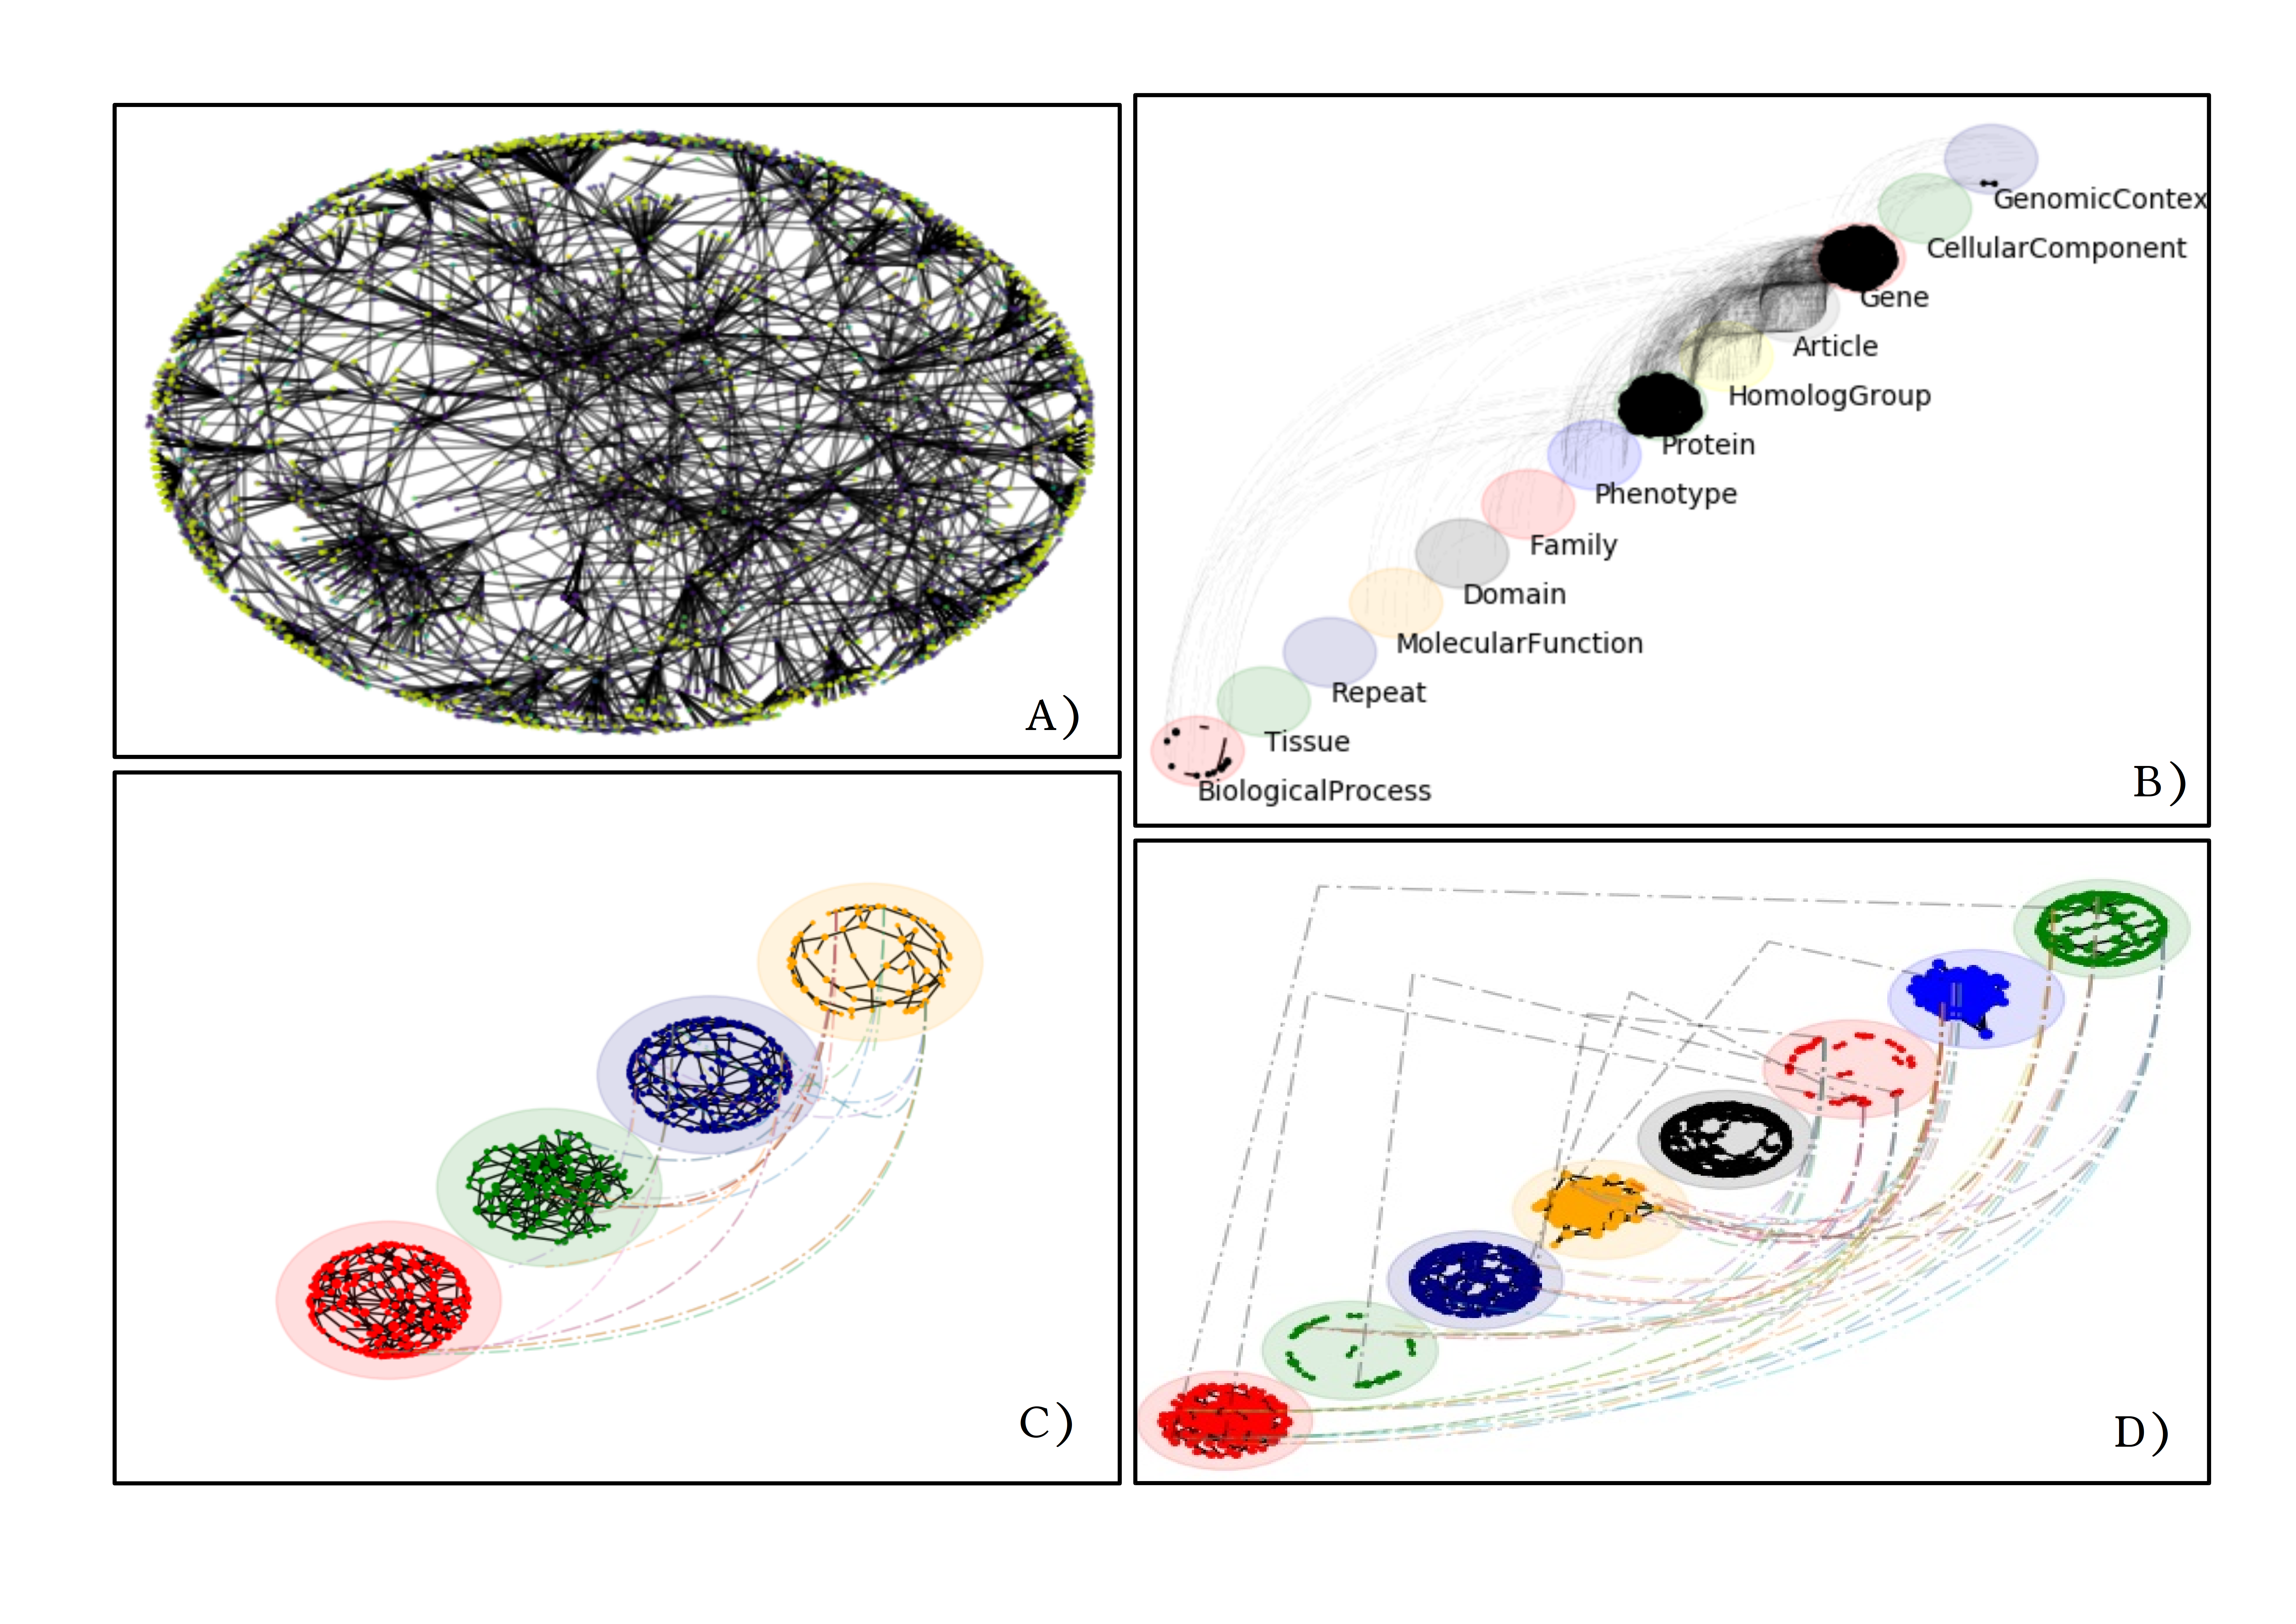
\includegraphics[width=1\textwidth]{images/test12.png}
\caption{Demonstration of Py3plex visualization capabilities. Visually incomprehensible network in A can be visualized using multiple layers, interconnected with smooth curves (B, C, D). This way, number of individual node types and their connectivity patterns are apparent. In B individual nodes are binned into layers by their coloring and thus visually comprehensible, whereas in A node types with lower frequencies can not be distinguished. The C and D demonstrate, that apart from connections (of more types) between individual types of nodes, topological patterns of individual layers can also be observed.}
\label{mainfig}
\end{figure}

\section{The Py3plex library}
We developed a lightweight Python library, capable of visualizing both the inter-layer node organization along with intra-layer connections between different types of nodes. As Py3plex is built on top of NetworkX, all layout, coloring and size properties can easily be transferred to a multiplex network from individual, single-layer networks. Example Py3plex visualizations are presented in Fig.\ref{mainfig}. The proposed implementation provides the abstractions, necessary to easily represent both the inter-layer properties (e.g. node clustering), as well as inter-layer connections in an intuitive manner. 

The Fig.1 depicts an example, how a complex, single-layer heterogeneous network obtained using BioMine network generator \cite{eronen2012biomine} can be separated into multiple layers, represented by parameterized second order Bernstein polynomials of the form
\begin{equation}
B(t) = (1 - t)^{2} P_{0} + 2(1-t)tP_{1}+t^{2}P_{2}; 0 \leq t \leq 1,
\end{equation}

where the $P_{0,1,2}$ represent the control points of an individual curve. In order to control the curve height, we added an additional term $\tau$, the equation 1 thus becomes:
\begin{equation}
B_{\tau}(t) = (1 - t)^{2} P_{0} \tau + 2(1-t)tP_{1}+t^{2}P_{2}; 0 \leq t \leq 1.
\end{equation}
The $\tau$ parameter thus enables additional optimization of multi-layer edge position. With larger $\tau$ values, multiplex edge is positioned further from the main layer diagonal.

The algorithm, which determines the optimal curve position is based on a simple triangulation procedure, where $P_{1}$ and $P_{3}$ represent the source and target node. The $P_{2}$ represents a point, located between $P_{1,3}$, which lies at the line, orthogonal to the $P_{1,3}$ line at height (or depth) $\tau$. Py3plex also supports many different styles of multiplex edge visualization; curve-based, triangle-based and simple line-based. 

\section{Conclusions}
Our contribution provides the means to visualize complex, heterogeneous networks in an intuitive manner, and is especially targeted at visualization of networks with multiple node types and many inter-layer edges. As it is built on top of a well established visualization library, it already supports extensive layout, coloring and shape options.

\begin{acknowledgements}
This work was founded by the Slovenian research agency (ARRS
\end{acknowledgements}


\bibliography{references}   % name your BibTeX data base
\bibliographystyle{apalike}  

\end{document}
% end of file template.tex

